%%%%%%%%%%%%%%%%%%%%%%%%%%%%%%%%%%%%%%%%%%%%%%%%%%%%%%%%%%%%%%%%%%%%%%%%%%%%%%%%
% TUM-Vorlage: Praesentation
%%%%%%%%%%%%%%%%%%%%%%%%%%%%%%%%%%%%%%%%%%%%%%%%%%%%%%%%%%%%%%%%%%%%%%%%%%%%%%%%
\input{./Ressourcen/Praesentation/Praeambel16zu9.tex} % Seitenverhaeltnis 16:9
\input{./_Einstellungen.tex}

\renewcommand{\PersonVorname}{David}
\renewcommand{\PersonNachname}{Gallob}

\usepackage{csquotes}
\usepackage[backend=biber,style=numeric,sorting=none]{biblatex} % Stil nach Wahl
\usepackage{hyperref}
\addbibresource{resources.bib} % Hier MIT Dateiendung .bib

\input{./Ressourcen/Praesentation/Anfang.tex}

\renewcommand{\LehrstuhlName}{Chair of Connected Mobility}
\renewcommand{\FakultaetName}{School of Computation, Information and Technology}

\title{Final Presentation --- A DSA-Compliant Tourism RS}
\subtitle{Final Presentation --- A DSA-Compliant Tourism Recommender System}
\author{David Gallob}
\institute[]{\UniversitaetName \\ \FakultaetName \\ \LehrstuhlName}
\date[July 6, 2026]{Munich, July 6, 2026}
\subject{Lab Course: Projects in Recommender Systems}
\PraesentationMasterStandard
\PraesentationTitelseite

% Slide 1: Introduction & Motivation
\begin{frame}
    \frametitle{Introduction \& Motivation}
    \begin{itemize}
        \item \textbf{The Recommender "Black Box":}
            \begin{itemize}
                \item Most modern recommender systems (RS) hide their inner workings (e.g. neural network rankings)~\cite{adomavicius2005toward, BORRAS20147370}.
                \item Causes user distrust, especially in high-stake domains like tourism (travel planning, hotel bookings)~\cite{ricci2011travel, knijnenburg2012explaining}.
            \end{itemize}
        \item \textbf{Regulatory Requirements: EU Digital Services Act (DSA)~\cite{eudsa2022}:}
            \begin{itemize}
                \item \textbf{Article 27:} Mandates that platforms explain the main parameters of their RS in plain, understandable language.
                \item \textbf{Article 38:} Mandates that Very Large Online Platforms (VLOPs) offer at least one profiling-free recommendation alternative.
            \end{itemize}
        \item \textbf{Project Goal:} Design and build an interactive, transparent, and DSA-compliant tourism recommender system prototype.
    \end{itemize}
\end{frame}

% Slide 2: Background: Recommender Systems in Tourism (NEW)
\begin{frame}
    \frametitle{Background: Recommender Systems in Tourism}
    \begin{itemize}
        \item \textbf{Unique Domain Characteristics~\cite{ricci2011travel, BORRAS20147370}:}
            \begin{itemize}
                \item High financial risk and emotional investment.
                \item Infrequent purchasing decisions (trips are planned only once or twice a year).
                \item Multi-attribute search spaces (price, location, stars, transport, amenities).
            \end{itemize}
        \item \textbf{Decision Complexity~\cite{ricci2011travel, BORRAS20147370}:}
            \begin{itemize}
                \item Unlike low-cost retail products (e.g. movies, books), users do not buy travel packages on impulse.
                \item Users require active comparison tools and want to express precise trade-offs.
                \item Trust and perceived control over the algorithm are essential for user acceptance~\cite{knijnenburg2012explaining}.
            \end{itemize}
    \end{itemize}
\end{frame}

% Slide 14: Demonstration
\PraesentationMasterWeissBlau
\begin{frame}
    \begin{center}
        \huge Solution
        \vspace{1em}
        \large Multiple Algorithms including explanations
    \end{center}
\end{frame}
\PraesentationMasterStandard
% Slide 13: Detailed System Architecture & Implementation (NEW)
\begin{frame}
    \frametitle{Two Algorithms with user defined weights/limits}
    \begin{columns}
        \begin{column}{0.53\textwidth}
    \begin{itemize}
        \item \textbf{5 Attributes for Hotels:}
            \begin{itemize}
                \item price per night, distance to center, stars, public transport access, user rating
            \end{itemize}
        \item \textbf{Two Algorithms:}
            \begin{itemize}
                \item \textbf{Weighted MAUT:} compensatory approach with user defined weights.
                \item \textbf{Constraint-Guided:} Focused on hard limit rules and non-compensatory filtering.
            \end{itemize}
    \end{itemize}
\end{column}
\begin{column}{0.43\textwidth}
            \begin{center}
                
\includegraphics[width=0.9\textwidth,keepaspectratio]{screens/Sliders.png}
                \begin{figure}
                    \tiny\caption{Dashboard}
                \end{figure}
            \end{center}
        \end{column}
    \end{columns}
\end{frame}

\begin{frame}
    \frametitle{System Architecture \& Technical Stack}
    \begin{itemize}
        \item \textbf{Technology Stack:}
            \begin{itemize}
                \item React\footnote{\url{https://react.dev/}} for component-based reactive state rendering.
                \item Vite\footnote{\url{https://vite.dev/}} as a fast bundler and build system.
                \item Vanilla CSS for a custom, glassmorphic design language.
                \item Client-side KaTeX\footnote{\url{https://katex.org/}} rendering for mathematical formulas.
            \end{itemize}
        \item \textbf{Real-Time Computation Flow:}
            \begin{itemize}
                \item Eliminates the latency of database queries. Real-time updates occur client-side as users drag the sliders.
                \item Caches the hotel calculations, avoiding unnecessary re-renders.
                \item Normalization boundaries recalculate dynamically upon city changes.
            \end{itemize}
        \item \textbf{Quality Assurance \& Verification:}
            \begin{itemize}
                \item Standalone recommender engine (\texttt{src/recommenderEngine.js}).
                \item 60 automated unit tests (\texttt{run-tests.js}) verifying edge cases, boundary conditions, and preventing division-by-zero errors.
            \end{itemize}
    \end{itemize}
\end{frame}

% Slide 6: Interactive Selection Wizard
\begin{frame}
    \frametitle{Interactive Landing Page for Algorithm Selection}
    \begin{columns}
        \begin{column}{0.53\textwidth}
    \begin{itemize}
        \item \textbf{Algorithmic State Initialization:}
            \begin{itemize}
                \item Recommendations, transparency boards, and controls are hidden initially to prevent cognitive overload.
            \end{itemize}
        \item \textbf{Two Strategy Selection Cards:}
            \begin{itemize}
                \item \textbf{Weighted MAUT Card:} Focused on relative importance weighting and compensatory trade-offs.
                \item \textbf{Constraint-Guided Card:} Focused on hard limit rules and non-compensatory filtering.
            \end{itemize}
        \item \textbf{Strategy Switching:}
            \begin{itemize}
                \item Simple back button ("← Switch Algorithm") to return to the landing page.
                \item Fast toggle tabs in the dashboard header for seamless switching.
            \end{itemize}
    \end{itemize}
\end{column}
\begin{column}{0.43\textwidth}
            \begin{center}
                
\includegraphics[width=0.9\textwidth,keepaspectratio]{screens/landing-page.png}
                \begin{figure}
                    \tiny\caption{User Weight Sliders (0-10 scale)}
                \end{figure}
            \end{center}
        \end{column}
    \end{columns}
\end{frame}

\begin{frame}
    \frametitle{Tiered Explainability \& Transparency Panels}
    \begin{columns}
        \begin{column}{0.48\textwidth}
            \begin{itemize}
                \item \textbf{Tier 1: Dynamic Banners (Plain Text)}
                    \begin{itemize}
                        \item Dynamic color schemes (Blue for MAUT, Green for Filtering).
                        \item Brief, plain-language summaries explaining how weights/limits are aggregated.
                    \end{itemize}
                \item \textbf{Tier 2: Algorithmic Details (TeX)}
                    \begin{itemize}
                        \item Expandable KaTeX mathematical formulas for expert review and full algorithmic disclosure.
                    \end{itemize}
                \item \textbf{Tier 3: Step-by-Step Breakdown}
                    \begin{itemize}
                        \item On-demand card expansions showing exact computations (Normalization $\times$ Weight).
                    \end{itemize}
            \end{itemize}
        \end{column}
        \begin{column}{0.48\textwidth}
            \begin{center}
                
\includegraphics[width=0.7\textwidth,keepaspectratio]{screens/Calculations.png}
                \begin{figure}
                    \tiny\caption{Step-by-Step Mathematical Breakdown}
                \end{figure}
            \end{center}
        \end{column}
    \end{columns}
\end{frame}

% Slide 14: Demonstration
\PraesentationMasterWeissBlau
\begin{frame}
    \begin{center}
        \huge Demonstration
        \vspace{1em}
        \large Real-Time Strategy Toggling \& Weight Adjustments
    \end{center}
\end{frame}
\PraesentationMasterStandard

% Slide 5: Initial UI Challenges & User Redesign (Moved to slide 13)% Slide 7: Algorithmic Strategy A: Weighted MAUT
\begin{frame}
    \frametitle{Algorithm A: Weighted MAUT (Compensatory)}
    \begin{columns}
        \begin{column}{0.53\textwidth}
            \begin{itemize}
                \item \textbf{Compensatory Utility Scoring~\cite{schmitt2002maut}:}
                    \begin{itemize}
                        \item Attributes: Price, Location, Stars, Guest Review, Transport.
                        \item Allows high performance in one attribute (e.g. location) to compensate for low performance in another (e.g. price).
                    \end{itemize}
                \item \textbf{Weights on a 0-10 Scale:}
                    \begin{itemize}
                        \item Range: $0$ (completely unimportant) to $10$ (most important).
                        \item Mathematically normalized by the total sum of user-specified weights:
                    \end{itemize}
            \end{itemize}
            \vspace{-0.2em}
            \begin{equation*}
              U = \frac{\sum w_i \cdot u_i}{\sum w_i} \times 100\%
            \end{equation*}
            \vspace{0.2em}
            \centering \tiny ($w_i$: attribute weight [0--10], $u_i$: normalized utility [0--1], $U$: match score \%)
        \end{column}
        \begin{column}{0.43\textwidth}
            \begin{center}
                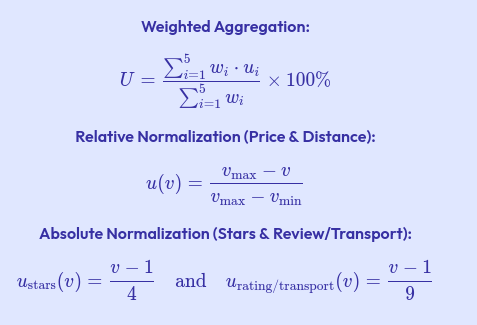
\includegraphics[width=0.9\textwidth,keepaspectratio]{screens/math.png}
                \begin{figure}
                    \tiny\caption{User Weight Sliders (0-10 scale)}
                \end{figure}
            \end{center}
        \end{column}
    \end{columns}
\end{frame}

% Slide 8: Normalization Strategies in MAUT (NEW)
\begin{frame}
    \frametitle{Normalization Strategies in Weighted MAUT}
    To aggregate attributes with different units, they are normalized to a $0-1$ scale~\cite{keeney1993decisions}:
    \begin{itemize}
        \item \textbf{Relative Normalization (Cost attributes: Price, Distance):}
            \begin{itemize}
                \item Normalizes value $v$ relatively based on the active city's min/max values:
            \end{itemize}
            \begin{equation*}
              u(v) = \frac{v_{\max} - v}{v_{\max} - v_{\min}}
            \end{equation*}
            \item Normalizing cost relatively maximizes the contrast between the local hotel options.
        \item \textbf{Absolute Normalization (Benefit attributes: Stars, Rating, Transit):}
            \begin{itemize}
                \item Normalizes value $v$ on fixed scale bounds to prevent artificial distortion:
            \end{itemize}
            \begin{equation*}
              u_{\text{stars}}(v) = \frac{v - 1}{4} \quad \text{and} \quad u_{\text{rating/transport}}(v) = \frac{v - 1}{9}
            \end{equation*}
    \end{itemize}
\end{frame}

% Slide 9: Algorithmic Strategy B: Constraint Filtering
\begin{frame}
    \frametitle{Algorithm B: Constraint-Based Filtering}
    \begin{columns}
        \begin{column}{0.48\textwidth}
            \begin{itemize}
                \item \textbf{Non-Compensatory Logic~\cite{ricci2011travel}:}
                    \begin{itemize}
                        \item User defines absolute thresholds (e.g. maximum price, minimum stars).
                        \item A hotel must satisfy all active limits simultaneously to be recommended.
                        \item Over-performing in one area cannot compensate for a single constraint violation.
                    \end{itemize}
                \item \textbf{DSA-Compliant Simplicity:}
                    \begin{itemize}
                        \item Unordered subset of matching hotels.
                        \item Easy-to-understand inclusion/exclusion criteria.
                        \item Complete profiling-free predictability.
                    \end{itemize}
            \end{itemize}
        \end{column}
        \begin{column}{0.48\textwidth}
            \begin{center}
                
\includegraphics[width=\textwidth,keepaspectratio]{screens/Constraint.png}
                \begin{figure}
                    \tiny\caption{Constraint Filtering Interface}
                \end{figure}
            \end{center}
        \end{column}
    \end{columns}
\end{frame}

% Slide 10: Non-Compensatory Satisficing Model (NEW)
\begin{frame}
    \frametitle{The Satisficing Model of Constraint Filtering}
    \begin{itemize}
        \item \textbf{Logical Conjunction Formulations:}
            \begin{itemize}
                \item A hotel is recommended if and only if:
            \end{itemize}
            \begin{equation*}
              \text{Price} \le P_{\max} \ \land \ \text{Distance} \le D_{\max} \ \land \ \text{Stars} \ge S_{\min} \ \land \ \text{Rating} \ge R_{\min} \ \land \ \text{Transport} \ge T_{\min}
            \end{equation*}
        \item \textbf{Psychological Background (Satisficing):}
            \begin{itemize}
                \item Based on Herbert Simon's bounded rationality theory (1957).
                \item Decision-makers do not seek the mathematically optimal hotel, but rather a "good enough" hotel that meets all minimal conditions.
                \item Drastically reduces cognitive load during selection.
                \item Perfect for users with rigid conditions (e.g., maximum budget).
            \end{itemize}
    \end{itemize}
\end{frame}

\begin{frame}
    \frametitle{UI Redesign \& User Experience Challenges}
    \vspace{1em}
    \begin{columns}
        \begin{column}{0.48\textwidth}
            \textbf{Initial Usability Issues:}
            \begin{itemize}
                \item Implicit strategy selection (no clear entry point).
                \item Cluttered landing state with premature disclosure of complex DSA transparency panels.
                \item Sliders scaled from $0-100\%$, confusing users into thinking weights must sum to $100\%$.
            \end{itemize}
            \vspace{0.5em}
            \textbf{Applied Redesign:}
            \begin{itemize}
                \item \textbf{Interactive Strategy:} landing page.
                \item Importance scale changed to \textbf{0-10 range} to prevent percentage-summing confusion.
            \end{itemize}
        \end{column}
        \begin{column}{0.48\textwidth}
            \begin{center}
                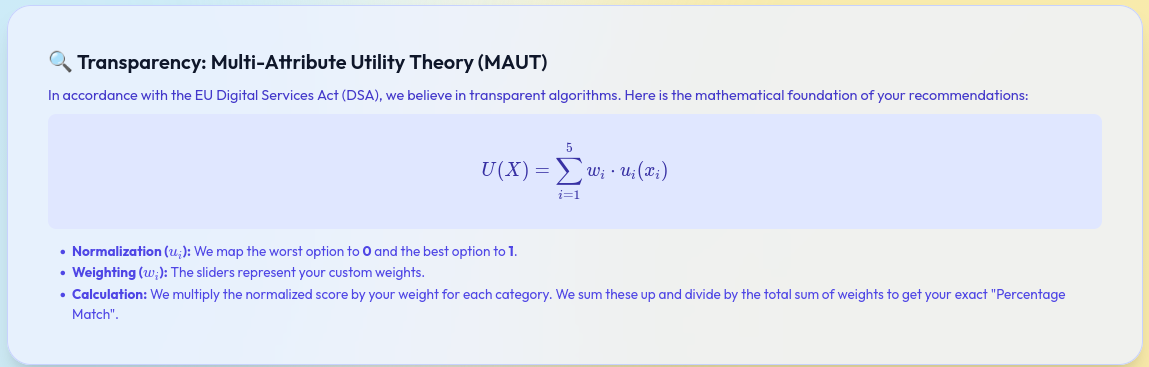
\includegraphics[width=0.9\textwidth,keepaspectratio]{screens/AlgoInfo.png}
                \begin{figure}
                    \tiny\caption{Previous Cluttered Transparency Board}
                \end{figure}
            \end{center}
        \end{column}
    \end{columns}
\end{frame}

% Slide 12: Tiered Explanation Design Theory (NEW)
\begin{frame}
    \frametitle{Different Explanation Levels}
    \begin{itemize}
        \item \textbf{The Explanation Dilemma~\cite{tintarev2012evaluating}:}
            \begin{itemize}
                \item Giving too little explanation makes the system look like a black box.
                \item Giving too much explanation causes cognitive overload and user fatigue.
            \end{itemize}
        \item \textbf{Tiered Disclosure (Satisfying Different User Persona):}
            \begin{itemize}
                \item \textbf{Novice Pathway (Banners):} Brief text explanations focusing on the meaning of user controls. Satisfies general transparency.
                \item \textbf{Expert Pathway (KaTeX Formulas):} Raw equations. Satisfies transparency audits and regulators.
                \item \textbf{Curious Pathway (Math Breakdown):} Step-by-step breakdown. Explains individual recommendations, boosting user trust.
            \end{itemize}
    \end{itemize}
\end{frame}
% Slide 11: Tiered Explainability Features (Moved to slide 14)% Future Work: Hybrid Recommender Slide
\begin{frame}
    \frametitle{Future Work: Proposed Hybrid Recommender}
    Addresses individual limitations of MAUT and Filtering:
    \begin{itemize}
        \item \textbf{Limitation of Weighted MAUT:} Compiles complete lists; does not filter out completely irrelevant options (e.g. extremely expensive hotels).
        \item \textbf{Limitation of Constraint Filtering:} Screens items but does not rank remaining candidates (higher cognitive effort).
    \end{itemize}
    \vspace{0.5em}
    \textbf{Proposed Two-Stage Hybrid Approach:}
    \begin{enumerate}
        \item \textbf{Stage 1: Constraint Filtering (Non-Compensatory screening):} Filter out hotels violating basic requirements (e.g. price $> \$250$).
        \item \textbf{Stage 2: Weighted MAUT (Compensatory ranking):} Apply preference weights to rank remaining candidates.
    \end{enumerate}
    \vspace{0.5em}
    $\Rightarrow$ Maintains complete mathematical transparency, remains profiling-free, and mimics realistic human decision-making.
\end{frame}

% Slide 15: Future Evaluation Design
\PraesentationMasterStandard
\begin{frame}
    \frametitle{Proposed User Study \& Evaluation Design}
    \begin{itemize}
        \item \textbf{Hypotheses:}
            \begin{itemize}
                \item \textbf{H1 (Perceived Control):} Users interacting with the Weighted MAUT or Constraint Filtering interfaces report a higher sense of control over recommendations compared to a baseline "black-box" interface.
                \item \textbf{H2 (System Trust):} Exposing the collapsible mathematical breakdown panels increases user trust in the system's recommendations without causing information overload.
                \item \textbf{H3 (DSA Compliance Impact):} The presence of the global explanation banner and KaTeX formulas increases user comprehension of the algorithm's inner workings.
            \end{itemize}
        \item \textbf{Within-Subjects Laboratory Study ($N=30$):}
            \begin{itemize}
                \item \textbf{Condition 1 (Baseline):} Traditional black-box hotel list.
                \item \textbf{Condition 2 (Weighted MAUT):} Slider controls with collapsible breakdowns.
                \item \textbf{Condition 3 (Constraint Filtering):} Threshold sliders.
            \end{itemize}
    \end{itemize}
\end{frame}



% Slide 17: Summary & Conclusion
\begin{frame}
    \frametitle{Summary \& Conclusion}
    \begin{itemize}
        \item \textbf{Successfully Completed Deliverables:}
            \begin{itemize}
                \item Developed an interactive, responsive tourism recommender SPA (React + Vite).
                \item Redesigned selection flow with a strategy landing page to prevent early transparency board clutter.
                \item Configured sliders on an intuitive 0-10 scale to eliminate weight-summing misunderstandings.
                \item Integrated tiered explainability panels (plain-language summaries, LaTeX formulas, math breakdowns).
            \end{itemize}
        \item \textbf{Key Takeaway:}
            \begin{itemize}
                \item Demonstrates that EU DSA compliance (Article 27 \& 38) can be harmonized with rich user controls, mathematical transparency, and premium UI/UX aesthetics.
            \end{itemize}
    \end{itemize}
\end{frame}

% Final Slide
\PraesentationMasterWeissBlau
\begin{frame}
    \begin{center}
        \huge Thank you for your attention! \\
        \vspace{1em}
        \large Questions?
    \end{center}
\end{frame}

\PraesentationMasterStandard
\begin{frame}[allowframebreaks]
    \frametitle{References}
    \printbibliography
\end{frame}

\PraesentationMasterWeissBlau
\begin{frame}
    \begin{center}
        \huge Backup Slides
    \end{center}
\end{frame}
\PraesentationMasterStandard

% Slide 3: Traditional Recommendation Strategies (NEW)
\begin{frame}
    \frametitle{Traditional Recommender System (RS) Strategies}
    \begin{itemize}
        \item \textbf{Collaborative Filtering (CF):}
            \begin{itemize}
                \item Predicts preferences based on ratings from similar users.
                \item \textit{Limitations in Tourism:} Cold start problems (new hotels/infrequent travelers) and lacks explanatory power.
            \end{itemize}
        \item \textbf{Content-Based Filtering (CB):}
            \begin{itemize}
                \item Recommends items matching a user profile built from historical behavior.
                \item \textit{Limitations in Tourism:} Poor adaptability to sudden context changes (e.g. business trip vs. family vacation).
            \end{itemize}
        \item \textbf{Hybrid Systems~\cite{8308293, Sarkar2023}:}
            \begin{itemize}
                \item Combine CF and CB. However, they remain mathematical black boxes to the end-user.
                \item Hard to explain, violating transparency guidelines.
            \end{itemize}
    \end{itemize}
\end{frame}

% Slide 4: HCI User Control & Trust (NEW)
\begin{frame}
    \frametitle{HCI: The Importance of User Control \& Trust}
    \begin{itemize}
        \item \textbf{Being Accurate is Not Enough~\cite{mcnee2006being}:}
            \begin{itemize}
                \item Traditional metrics focus solely on algorithmic accuracy (e.g., RMSE).
                \item Ignores user factors like transparency, control, and serendipity.
            \end{itemize}
        \item \textbf{Beyond Algorithms~\cite{swearingen2001beyond}:}
            \begin{itemize}
                \item Interactive systems should give users a direct steering wheel.
                \item Sliders and constraints shift the role of the user from a passive consumer to an active co-creator.
            \end{itemize}
        \item \textbf{Explaining the User Experience~\cite{knijnenburg2012explaining}:}
            \begin{itemize}
                \item Combining user control with visual explanations leads to significantly higher trust, perceived recommendation quality, and system satisfaction.
            \end{itemize}
    \end{itemize}
\end{frame}

% Slide 16: Detailed Study Evaluation Metrics (NEW)
\begin{frame}
    \frametitle{Proposed User Study Evaluation Metrics}
    To scientifically test the hypotheses, standardized metrics will be gathered:
    \begin{itemize}
        \item \textbf{System Usability Scale (SUS):}
            \begin{itemize}
                \item 10-item Likert scale questionnaire to evaluate overall system usability.
            \end{itemize}
        \item \textbf{ResQue (Recommender Systems Quality of Experience)~\cite{knijnenburg2012explaining}:}
            \begin{itemize}
                \item Focuses on user-centric quality: perceived quality, system trust, transparency, and intent to use.
            \end{itemize}
        \item \textbf{NASA Task Load Index (NASA-TLX):}
            \begin{itemize}
                \item Focuses on subjective cognitive workload.
                \item Measures: Mental demand, physical demand, temporal demand, performance, effort, and frustration level. Helps verify if exposing math equations causes overload.
            \end{itemize}
    \end{itemize}
\end{frame}
\end{document}
